\documentclass[12pt]{article}
\usepackage{tikz}
\usepackage{circuitikz}
\usepackage{amsmath}
\usepackage{amssymb}
\usepackage{graphicx}
\usepackage{float}
\usepackage{geometry}
\usepackage{pgfplots}
\usepackage{color}
\usepackage{xcolor}

\geometry{a4paper, margin=1in}
\pgfplotsset{compat=1.18}

\begin{document}

Consider triangle ABC:

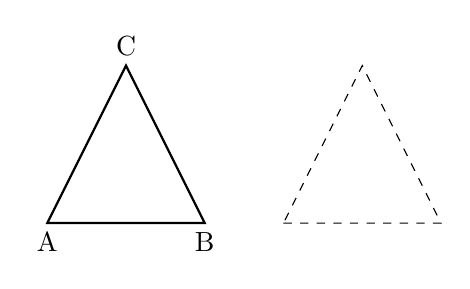
\begin{tikzpicture}
\draw[thick] (0,0) -- (2,0) -- (1,2) -- cycle;
\node[below] at (0,0) {A};
\node[below] at (2,0) {B};
\node[above] at (1,2) {C};
\draw[dashed] (3,0) -- (5,0) -- (4,2) -- cycle;
\end{tikzpicture}

The dashed triangle is a transformation of triangle ABC.
Identify the transformation and specify its parameters.

\end{document}
